\documentclass[a4paper, 11pt]{article}
\usepackage{preamble}
% \usepackage{fullpage}
\usepackage[paper=a4paper,margin=1.5in, includeheadfoot, footskip=30pt]{geometry}
\usepackage{dsfont}
\usepackage{algorithm}
\usepackage{algorithmic}
\usepackage{paralist}
\usepackage{csvsimple}
\usepackage{longtable}
\usepackage{booktabs}
\usepackage{tikz}
\usepackage{afterpage}
\usepackage{multicol}
\usepackage{cleveref}
\usepackage[toc]{appendix}

\hypersetup{
    colorlinks = false,
    linkbordercolor = 1 1 0,
}


\sisetup{range-phrase=-}
\DeclareSIUnit{\au}{a.u.}

\crefformat{footnote}{#2\footnotemark[#1]#3}

\newcommand{\drawfrom}{\overset{\mathrm{d}}{=}}
\newcommand{\setfrom}{\overset{\mathrm{d}}{\leftarrow}}


\title{ \small
University of Oslo\\
FYS4411\\
Computational physics II: Quantum mechanical systems\\
\huge Project 2: The Restricted Boltzmannn Machine Applied to the Quantum Many Body Problem}
\author{\textsc{Bendik Samseth}}
\date{\today}
\begin{document}
\maketitle

\begin{abstract}
    Abstract here, please.
    All material referenced in this report is available at
    \url{https://github.com/bsamseth/FYS4411}.
\end{abstract}


\pagebreak
\newgeometry{margin=0.9in}
\tableofcontents

\begin{multicols}{2}    

    \section{Introduction} 

    A physicist faced with a quantum many body system is quickly forced to
    abandon any hope of solving the Schrödinger equation (or one of its even worse
    relativistic siblings) exactly. Instead he must resort to one of two general
    workarounds: 1) make simplifying assumptions until the equation is solvable,
    or 2) make an educated guess for the solution. In either case, the desired
    quantity which solving the Schrödinger equation would yield is the quantum
    mechanical wavefunction. If we want to stay away from potentially faulty, or
    limiting assumptions, we must therefore somehow produce a guess for this
    wavefunction, without actually solving the equation.

    The last project utilized the Variational Monte Carlo (VMC) approach, in which a
    specific, parametrized form is assumed for the wavefunction, with the
    subsequent optimization of the parameters.

    The main limitation of VMC is that a specific form for the wavefunction is
    assumed. If this form contains the true optimum that works fine, but if not
    we are inherently limited in how accurate the final results can be.

    Aiming to be overcome this issue, we may observe that the task at hand falls
    into the general field of function approximation. We wish to approximate the
    function that takes as input the configuration of the system, and outputs a
    probability amplitude for the given state. Function approximation is a task
    which lends itself to techniques from machine learning (ML). 

    In this project we will attempt to represent the wavefunction with a
    specific type of ML-model, the Restricted Boltzmann Machine (RBM). The use
    of RBMs for such applications was presented recently by
    \textcite{Carleo602}, with encouraging results. We shall therefore attempt
    to apply the same techniques to a different type of system, namely that of
    two interacting quantum particles confined in a harmonic oscillator trap.


    \section{Theory}

    \subsection{The System}

    We consider a system of electrons confined in a pure two-dimensional
    isotropic harmonic oscillator potential, with an idealized total Hamiltonian
    given by:

    \begin{align}
        \begin{split}
            \hat H &= \sum_{i=1}^P\qty(-\frac{1}{2}\laplacian_i + V_{ext}(\vec r_i)) +
            \sum_{i < j} V_{int}(\vec r_i, \vec r_j)\\
            &= \sum_{i=1}^P\qty(-\frac{1}{2}\laplacian_i + \frac{1}{2}\omega^2
            r_i^2) + \sum_{i < j} \frac{1}{r_{ij}},
        \end{split}\label{eq:H-def}
    \end{align}
    where natural units ($\hbar=c=m_e=1$) are used with energies in
    atomic units (a.u.), $P$ denotes the number of particles in the system, and
    $\omega$ is the oscillator frequency of the trap. Further, $\vec r_i$
    denotes the position vector of particle $i$, with $r_i \equiv \norm{\vec r}$ and
    $r_{ij}\equiv \norm{\vec r_i - \vec r_j}$ defined for notational brevity.

    In this project we limit ourselves to the case of $N=2$ interacting
    electrons in a trap with a frequency such that $\hbar \omega = 1$. We do
    this because for this case we have exact, analytical solutions for the
    ground state energy. With the interaction term included, the ground state
    energy is $E_0 = \SI{3}{\au}$~\cite{Taut1993}. This limitation is purely one
    of convenience, as having exact benchmarks makes for better verification of
    results. The methods discussed in the project should extend to other
    systems.

    \subsection{Simple Non-Interacting Case}
    If we omit the interacting terms in \autoref{eq:H-def} we have
    the standard harmonic oscillator Hamiltonian:
    \begin{align}
        \hat H_0 &= \sum_{i=1}^P\qty(-\frac{1}{2}\laplacian_i +
        \frac{1}{2}\omega^2 r_i^2).
    \end{align}
    This Hamiltonian lends it self to analytical solutions, and the stationary
    states are:
    \begin{align}
        \phi_{n_x, n_y}(x, y) &= A H_{n_x}(\sqrt\omega x)H_{n_y}(\sqrt\omega y)
        e^{-\frac{\omega}{2}\qty(x^2 + y^2)},
    \end{align} 
    for quantum numbers $n_x, n_y = 0, 1,\dots$, and the Hermite polynomials
    $H_n$. The ground state, $n_x=n_y=0$ is simply
    \begin{align}
        \phi_{00}(x,y) =
        \sqrt{\frac{\omega}{\pi}}e^{-\frac{\omega}{2}\qty(x^2+y^2)}.
    \end{align}
    Using this wavefunction we can calculate the ground state
    energy\footnote{\label{fnt:sympy}See \texttt{projects/python/Sympy.ipynb} in the Github
    reposirepository for an explicit calculation of the ground state energy},
    \begin{align}
        \epsilon_{00} = \frac{\expval{\hat H_0}{\phi_{00}}}{\braket{\phi_{00}}}
        = \omega = \SI{1}{\au}
    \end{align}

    The ground state wavefunction for the (unperturbed) two-electron case is simply the
    product of the one-electron wavefunctions,
    \begin{align}
        \begin{split}
            \Phi(\vec r_1, \vec r_2) &= \phi_{00}(\vec r_1)\phi_{00}(\vec r_2)\\
            &= \frac{\omega}{\pi} e^{-\frac{\omega}{2}\qty(r_1^2+r_2^2)}.
        \end{split}\label{eq:Phi-non-inter}
    \end{align}

    The ground state energy can once again be evaluated
    analytically\cref{fnt:sympy} and yields
    \begin{align}
        E_0 = \frac{\expval{\hat H_0}{\Phi}}{\braket{\Phi}}
        = 2\omega =\SI{2}{\au}
    \end{align}
    This result is not surprising, as adding one more particle, without any
    interactions, should simply double the energy. Another way to look at it is
    that the simple harmonic oscillator solution gives $\flatfrac{\omega}{2}$
    per degree of freedom, so adding another two yields and extra $\omega$.


    When the two particles are electrons, we may say something about their total
    spin. As electrons are fermions, their total wavefunction must be
    anti-symmetric upon interchanging the labels $1$ and $2$.
    \autoref{eq:Phi-non-inter} is obviously symmetric, and so the
    spin-wavefunction must necessarily be anti-symmetric. For the combination of
    two spin-1/2 particles, there is only one candidate, namely the spin-0
    singlet:

    \begin{align}
        \chi_0 = \frac{1}{\sqrt 2}\qty(\ket{\uparrow\downarrow} -
        \ket{\downarrow\uparrow}).
    \end{align}

    \section{Representing the Wavefunction with an RBM}

    Our machine learning model of choice is the Restricted Boltzmann Machine. It
    consists of of two densely interconnected layers, the \emph{visible} layer
    and the \emph{hidden} layer. It is called restricted because we only
    connections between nodes in different layers - no visible-to-visible or
    hidden-to-hidden connections are included.

    The RBM is a generative model, meaning it learns a probability distribution
    for its inputs. This means that a trained RBM can produce outputs which
    when viewed as a distribution, would be similar to the distribution of the
    inputs. For our case, this means learning the probability distribution for
    the space configurations of the electrons in our system. We may interpret
    this distribution as the wavefunction, as the wavefunction serves this same
    purpose.

    In this case we do not have a training set of positions for any of the
    systems under consideration. This means that the most desired training
    regime, \emph{supervised training}, is not relevant for our problem. Instead
    we shall use \emph{reinforcement training}, were updates of the model are
    based on the variational principle: The true ground state wavefunction is
    the wavefunction for which the lowest ground state energy is obtained. We
    can treat the energy a certain wavefunction (model configuration) produces
    as the penalty, and let the model adapt as to minimize the penalty it
    receives.
    
    \subsection{The Math}
    
    In the following, $\vec x$ denotes the values of the visible layer (our
    position coordinates), and $\vec h$ denotes the values of the hidden layer.

    The joint probability distribution over $\vec x$ and $\vec h$ is:
    \begin{align}
        F_{RBM}(\vec x, \vec h) = \frac{1}{Z} e^{-\frac{1}{T_0}E(\vec x, \vec
        h)}\label{eq:F-RBM-def},
    \end{align}
    where $Z$ is the partition function ensuring that $F_{RBM}$ is normalized.
    In accordance with common norm, we set $T_0=1$. The function $E(\vec x, \vec
    h)$ is known as the energy of a configuration of the nodes, not to be
    confused with the energy of the quantum system. It encodes the probability
    of a given configuration - high energy configurations are less likely.

    \subsubsection{Gaussian-Binary RBM}

    The type of energy function we will use is called Gaussian-Binary, meaning
    our inputs (the position coordinates) are Gaussian (continuous), while the
    hidden nodes take binary values $h_j\in \{0, 1\}$. It looks as follows:
    \begin{align}
        E(\vec x, \vec h) = \frac{\norm{\vec x-\vec a}}{2\sigma^2} - \vec
        b^T\vec h - \frac{\vec x^T\vec w \vec h}{\sigma^2},
    \end{align}
    where $\vec a\in \mathbf{R}^M, \vec b\in \mathbf{R}^N$ are bias vectors for the visible and hidden layers
    respectively, and $\vec w\in \mathbf{R}^{M\times N}$ is a matrix encoding
    the weights for every connection between the two layers.
    In our case, $M=PD$ for $P$ particles in $D$ dimensions, while $N$ will be
    chosen freely by us.

    \subsubsection{The Wavefunction}

    The wavefunction is:
    \begin{align*}
        \Psi(\vec X) &= F_{RBM}(\vec x) = \sum_{\vec{h}} F_{RBM}(\vec x, \vec h)\\
        &=\frac{1}{Z} e^{-\sum_i^M \frac{\qty(X_i-a_i)^2}{2\sigma^2}}
        \prod_j^N \qty(1 + e^{b_j+\sum_i^M \frac{X_iw_{ij}}{\sigma^2}})\\
        &\equiv \frac{1}{Z}e^{-\sum_i^M
        u_i}\prod_j^N(1+e^{v_j})\numberthis\label{eq:Psi-def}
    \end{align*}
    where $u_i$ and $v_j$ are defined for convenience.





    \section{The Cost Function - Energy}
    \subsection{Definition}

    The cost function we use to train the network shall be the expectation value
    of the Hamiltonian, under the wavefunction modeled by the network.
    Minimizing the energy will yield the best possible wavefunction obtainable
    within the model. The energy is expressed as
    \begin{align}
        Q = E[H] = \expval{H} = \frac{\int \dd{\vec X} \Psi^* \hat H \Psi}{\int
        \Psi^*\Psi}.
    \end{align}
    where $\vec X$ is the vector containing all the positions of the particles in
    the system, $\vec X = [x_1, y_1,\dots, x_n, y_n]$.
    In order to numerically evaluate this integral we first manipulate it a bit.
    The probability density at position $\vec X$, under the trial wave function, is
    \begin{align}
        P(\vec X) &= \frac{\abs{\Psi}^2}{\int \dd{\vec X}\abs{\Psi}^2}.
    \end{align}
    We finally define a new quantity, called \textbf{the local energy}:
    \begin{align}
        E_L(\vec X) &= \frac{1}{\Psi}\hat H\Psi\label{eq:E_L}
    \end{align}
    Combining these two definitions we can now rewrite $\expval{H}$ as follows:
    \begin{align}
        \begin{split}
            \expval{H} &= \int \dd{\vec X} P(\vec X) E_L(\vec X)\\
            &\approx
            \frac{1}{n}\sum_{i=1}^n E_L(\vec X_i),
        \end{split}\label{eq:the-objective}
    \end{align}
    where $\vec X_i$ are $n$ randomly drawn positions from the PDF $P(\vec X)$.
    We have therefore that estimating the average value of $E_L$ yields an
    approximated value for $\expval{H}$. 
    
    \subsection{Optimization}

    In order to train the model to minimize $\expval{\hat H}$ we need to know
    how to adjust the parameters $\vec\alpha = (a_1,\dots,a_M,
    b_1,\dots,b_N,w_{11},\dots,w_{MN})$. We do this using some optimization
    algorithm, which will in turn be based on the partial derivatives of the
    expectation of the local energy~\cite{mhj-compphys-II}:
    \begin{align}
            G_i &= \pdv{\expval{E_L}}{\alpha_i} 
            = 2\qty(\expval{E_L
        \frac{1}{\Psi}\pdv{\Psi}{\alpha_i}} -
        \expval{E_L}\expval{\frac{1}{\Psi}\pdv{\Psi}{\alpha_i}})
    \end{align}
    These partial derivatives are trivial to compute analytically, and come out as
    follows:
    \begin{align}
        \frac{1}{\Psi}\pdv{\Psi}{a_k} &=
        \frac{x_k-a_k}{\sigma^2}\label{eq:pdv-a}\\
        \frac{1}{\Psi}\pdv{\Psi}{b_k} &= \frac{1}{1 +
        e^{-v_k}}\label{eq:pdv-b}\\
        \frac{1}{\Psi}\pdv{\Psi}{w_{kl}} &= \frac{1}{1 +
        e^{-v_l}}\frac{x_k}{\sigma^2}
    \end{align}

    The expression for the local energy it self is a bit less trivial to work
    out, but still doable. And as we shall need to compute the local energy often,
    it will be useful to do the differentiation analytically, so as to speed up
    the computation compared to doing the second derivative in $\hat H$
    numerically. The details are laid out in \autoref{app:E-L-derivation}.

    The final expression we shall use for the local energy is:
    \begin{align}
        E_L &= \sum_{i=1}^M \frac{1}{2}x_i^2 + \sum_{i<j}^{P} \frac{1}{r_{ij}}
        - \frac{1}{2} \sum_{k=1}^M
        \frac{1}{\Psi}\pdv[2]{}{x_k}\Psi,\label{eq:E-L-final-main-section}
    \end{align}
    where,
    \begin{align}
        \begin{split}
        \frac{1}{\Psi}\pdv[2]{}{X_k}\Psi 
        &= -\frac{1}{\sigma^2} - \sum_j^N
        \frac{w_{kj}^2}{\sigma^4}
        \frac{e^{-v_j}}{\qty(1+e^{-v_j})} \\
        &\quad{   }\quad{      }  +
        \frac{1}{\sigma^4}\qty(-X_k+\sum_j^N \frac{w_{kj}}{1+e^{-v_j}})^2
        \end{split}
        \label{eq:E-L-second-deriv-main-section}
    \end{align}
    The complexity of $E_L$ is $\mathcal{O}(M + P^2 + MNM) = \mathcal{O}(P^2 +
    M^2 N)$. This can be optimized slightly by computing all the $v_j$ terms at
    once (as opposed to on demand within the sums), which brings this down to
    $\mathcal{O}(P^2 + MN)$. It still scales quadratically with additional
    particles (and dimensions), and linearly with the number of hidden nodes.

    Comparing this with the results from project 1, where the complexity of a
    local energy evaluation was $\mathcal{O}(P^3)$ when a similar interaction
    was considered, we see a significant
    difference. \emph{Assuming} we can obtain good results using an RBM where $N$ is
    comparable to $P$ in size, this new approach has much better time-complexity
    and therefore looks much more promising for use with large systems. We will
    not pursue this large $P$ regime much further in this project, but this is
    something to note, if the RBM prove to be fruitful.

    \subsection{Regularization}

    We may wish to impose some regularization in the cost function as well.
    Often times this can help guide the optimization out of local minima, as
    well as shaping ill-formed cost functions. We can modify the cost function
    as follows:
    \begin{align}
        Q = \expval{H} + \gamma\norm{\vec \alpha}_d^d,
    \end{align} 
    where $\gamma>0$ is a hyper-parameter controlling the amount of
    regularization, and $\norm{\cdot}_d^d$ is the $L_d$ norm. Two of the most widely used
    types of regularization are Ridge and Lasso, which use $d=2$ and $d=1$,
    respectively. In order to keep the gradient simple, we will only implement
    Ridge loss. We obtain then a slightly modified form for $G_i$:
    \begin{align}
        G_i = \pdv{\expval{E_L}}{\alpha_i} +
        2\gamma\alpha_i,\label{eq:G-i-ridge}
    \end{align}



    \section{Results}

    \subsection{One Particle in One Dimension} 

    As a first test of the RBM, we apply it to the very simple simple case of a
    single particle in one dimension. We will use the standard metropolis
    sampling algorithm to begin with. \autoref{fig:rbm-1d-1p} shows the learned
    wavefunction after $\num{2e4}$ iterations, using a learning rate of $0.9$,
    and no regularization. The energy produced by this wavefunction comes out as
    $0.50033\pm \num{5.6e-6}\si{\au}$, compared to the exact value of
    $\SI{0.5}{\au}$. The error given here is the standard error of the mean
    local energy, as calculated with the Blocking method discussed in project 1,
    using $2^{15}$ samples. If we allow for more training, the energy is lower
    somewhat more, although the gains diminish as $E_L$ approaches its ideal
    value.

    Applying regularization in this case, for almost any reasonable choice for
    $\gamma$ (e.g. $0.1$), the RBM converges \emph{very} quickly to the exact
    wavefunction, by setting all parameters as small as possible. The effect of
    regularization is artificially magnified in this situation, as it so happens
    that the minimizing choice of parameters coincide with the minimizing choice
    for the regularization term, i.e the trivial $\vec\alpha=\vec 0$ solution.
    We cannot expect this to work as well for less trivial tests, but it serves
    as a nice sanity check for the developed codes.


\end{multicols}

\begin{figure}[ht]
    \centering
    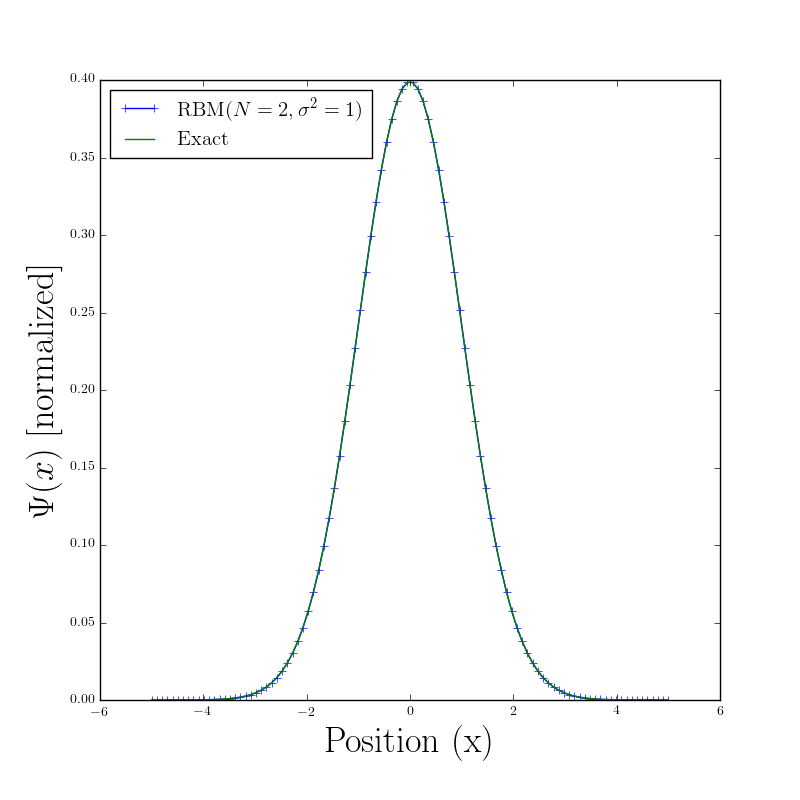
\includegraphics[width=0.8\linewidth]{../results/rbm-1d-1p.png}
    \caption{Ideal and learned wavefunction for one particle in one dimension.}
    \label{fig:rbm-1d-1p}
\end{figure}

\begin{multicols}{2}

    \printbibliography

\end{multicols}




\pagebreak
\begin{multicols}{2}
    \appendix
    \addcontentsline{toc}{section}{Appendices}
    \section*{Appendices}

    \section{Analytic Expression for the Local Energy}
    \label{app:E-L-derivation}
    
    To get started we will be needing a couple of partial derivatives:
   \begin{align}
        \pdv{}{X_k} (1+e^{v_j}) &=e^{v_j}\pdv{}{X_k}v_j =
        e^{v_j} \frac{w_{kj}}{\sigma^2}\\
        \begin{split}
        \pdv{}{X_k}e^{-\sum_i^M u_i} &= e^{-\sum_i^M
        u_i}\pdv{}{X_k}\qty(-\sum_i^M u_i) \\
        &= e^{-\sum_i^M u_i}\pdv{}{X_k} (-u_k) \\
        &= -e^{-\sum_i^M u_i} \frac{x_k-a_k}{\sigma^2}
        \end{split}
    \end{align}

    We are now ready to compute the first derivate:
    \begin{align*}
        \pdv{}{X_k}\Psi &= \frac{1}{Z} \left[\prod_j^N
        \qty(1+e^{v_j})\pdv{}{X_k}e^{-\sum_i^M u_i}\right.\\
        &\quad{  }\quad{    }\left. + e^{-\sum_i^M
        u_i}\pdv{}{X_k} \prod_j^N \qty(1+e^{v_j})\right]\\
        &= -\frac{x_k-a_k}{\sigma^2}\Psi + \Psi \sum_j^N
        \qty(\frac{1}{1+e^{v_j}}\pdv{}{X_k}\qty(1+e^{v_j}))\\
        &= -\frac{x_k-a_k}{\sigma^2}\Psi + \Psi\sum_j^N
        \frac{1}{1+e^{v_j}}\qty(\frac{w_{kj}}{\sigma^2} e^{v_j})\\
        &= \frac{1}{\sigma^2}\qty(a_k-x_k + \sum_j^N
        \frac{w_{kj}}{1+e^{-v_j}})\Psi.
    \end{align*}

    Before jumping into the second derivative, one more helpful derivative:
    \begin{align}
        \begin{split}
        \pdv{}{X_k}\qty(\frac{w_{kj}}{1+e^{-v_j}}) &=
            w_{kj}\frac{e^{-v_j}}{\qty(1+e^{-v_j})^2}\pdv{(-v_j)}{X_k}\\
        &= -\frac{w_{kj}^2}{\sigma^2} \frac{e^{-v_j}}{\qty(1+e^{-v_j})}
        \end{split}
    \end{align}

    Now, finally the second derivative:
    \begin{align*}
        \frac{1}{\Psi}\pdv[2]{}{X_k}\Psi &= \frac{1}{\Psi}\pdv{}{X_k}\qty[\frac{1}{\sigma^2}\qty(a_k-x_k + \sum_j^N
        \frac{w_{kj}}{1+e^{-v_j}})\Psi]\\
        &= \frac{1}{\sigma^2} \left[ \pdv{}{X_k}\qty(a_k-x_k + \sum_j^N
        \frac{w_{kj}}{1+e^{-v_j}} )   \right.\\
        &\quad{   }\quad{   } \left. 
        + \qty(a_k-x_k + \sum_j^N
        \frac{w_{kj}}{1+e^{-v_j}})\frac{1}{\Psi}\pdv{}{X_k}\Psi 
        \right]\\
        \begin{split}
        &= -\frac{1}{\sigma^2} - \sum_j^N
        \frac{w_{kj}^2}{\sigma^4}
        \frac{e^{-v_j}}{\qty(1+e^{-v_j})} \\
        &\quad{   }\quad{      }  +
        \frac{1}{\sigma^4}\qty(a_k-x_k+\sum_j^N \frac{w_{kj}}{1+e^{-v_j}})^2
        \end{split}\numberthis\label{eq:E-L-second-deriv}
    \end{align*}


    The final expression we shall use then for the local energy is:

    \begin{align}
        E_L &= \sum_{i=1}^P \frac{1}{2}r_i^2 + \sum_{i<j}^{P} \frac{1}{r_{ij}}
        - \frac{1}{2} \sum_{k=1}^M
        \frac{1}{\Psi}\pdv[2]{}{x_k}\Psi,\label{eq:E-L-final}
    \end{align}
    substituting in \autoref{eq:E-L-second-deriv}.

\end{multicols}



\end{document}
